\documentclass[a4paper,12pt]{article} 

%%% Работа с русским языком
\usepackage{cmap}					% поиск в PDF
\usepackage{mathtext} 				% русские буквы в фомулах
\usepackage[T2A]{fontenc}			% кодировка
\usepackage[utf8]{inputenc}			% кодировка исходного текста
\usepackage[english,russian]{babel}	% локализация и переносы

%%% Дополнительная работа с математикой
\usepackage{amsmath,amsfonts,amssymb,amsthm,mathtools, gensymb} % AMS
\usepackage{icomma} % "Умная" запятая: $0,2$ --- число, $0, 2$ --- перечисление

%%Таблица
\usepackage[table,xcdraw]{xcolor}
\usepackage{caption}
\usepackage{floatrow}
\floatsetup[table]{capposition=top}
\floatsetup[wrapfigure]{capposition=bottom}

%Отступы и поля 
\textwidth=18cm
\oddsidemargin=-1cm
\topmargin=-2cm
\textheight=25cm


%% Номера формул
\mathtoolsset{showonlyrefs=true} % Показывать номера только у тех формул, на которые есть \eqref{} в тексте.

%% Шрифты
\usepackage{euscript}	 % Шрифт Евклид
\usepackage{mathrsfs} % Красивый матшрифт

%% Свои команды
\DeclareMathOperator{\sgn}{\mathop{sgn}}

%% Перенос знаков в формулах (по Львовскому)
\newcommand*{\hm}[1]{#1\nobreak\discretionary{}
{\hbox{$\mathsurround=0pt #1$}}{}}

%% Стиль страницы
\usepackage{fancyhdr}

%% Для рисунков
\usepackage{graphicx}
\usepackage[export]{adjustbox}
\usepackage{float}
\usepackage{ragged2e}
\usepackage{wrapfig}

\pagestyle{fancy}
\begin{document}
\begin{titlepage}
\begin{center}
%\vspace*{1cm}
\large{\small ФЕДЕРАЛЬНОЕ ГОСУДАРСТВЕННОЕ АВТОНОМНОЕ ОБРАЗОВАТЕЛЬНОЕ\\ УЧРЕЖДЕНИЕ ВЫСШЕГО ОБРАЗОВАНИЯ \\ МОСКОВСКИЙ ФИЗИКО-ТЕХНИЧЕСКИЙ ИНСТИТУТ\\ (НАЦИОНАЛЬНЫЙ ИССЛЕДОВАТЕЛЬСКИЙ УНИВЕРСИТЕТ)\\ ФАКУЛЬТЕТ АЭРОКОСМИЧЕСКИХ ТЕХНОЛОГИЙ}
\vfill
\line(1,0){490}\\[1mm]
\huge{Лабораторная работа 4.9}\\
\huge\textbf{Исследование гальванометра}\\
\line(1,0){490}\\[1mm]
\vfill
\begin{flushright}
\normalsize{Рогозин Владимир}\\
\normalsize{\textbf{Группа Б03-106}}\\
\end{flushright}
\end{center}
\end{titlepage}
\fancyhead[L] {Работа 4.9}


\textbf{Цель работы}: изучение работы высокочувствительного зеркального
гальванометра магнитоэлектрической системы в режимах измерения постоянного тока и электрического заряда.

\textbf{Оборудование}: зеркальный гальванометр с осветителем и шкалой, источник постоянного напряжения, делитель напряжения, магазин сопротивлений, эталонный
конденсатор, вольтметр, переключатель, ключи, линейка.

\textbf{Теоретические сведения}: Гальванометром называют электроизмерительный прибор высокой чувствительности. С его помощью измеряют малые токи, напряжения, заряды, магнитные потоки. 

\begin{wrapfigure}[12]{l}{0.4\textwidth}\label{fig: diod}
    \begin{center}
    \vspace{-20pt}
        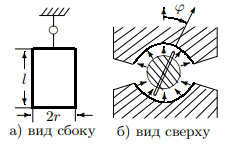
\includegraphics[width = 0.8\textwidth]{рамкаВМагните.png}
    \end{center}
    \caption{Рамка с током в магнитном поле}
\end{wrapfigure}
Главной частью высокочувствительного гальванометра магнитоэлектрической
системы является подвешенная на вертикальной нити рамка, помещённая в поле
постоянного магнита. Вырез цилиндрической формы в полюсах магнита и ферромагнитный цилиндр на оси системы делают поле в зазоре радиальным. Скреплённое с рамкой зеркальце служит для измерения угла поворота рамки. 

Гальванометр магнитоэлектрической системы с большим периодом колебаний ($T > 10 \text{ с}$) называют баллистическим. К рамке баллистического гальванометра прикреплён полый цилиндр, который сильно увеличивает момент инерции и, следовательно, период колебаний подвижной системы, не очень её утяжеляя. Баллистический гальванометр позволяет измерять как постоянный ток (стационарный или динамический режим), так и заряд, протекший через рамку за некоторое время (баллистический режим). В баллистическом режиме гальванометр может работать, если время протекания заряда много меньше периода собственных колебаний подвижной рамки. Поэтому период колебаний рамки делают большим.
Это время учитывает также реакцию экспериментатора, которому надо успеть сделать отсчёт максимального отклонения рамки.

\textbf{Уравнение движения подвижной системы.} На помещённую в магнитное поле обтекаемую током рамку гальванометра действуют следующие моменты сил: момент закрученной нити, момент магнитных сил и тормозящий момент, зависящий от сил сопротивления воздуха и от индукционных токов, вызывающих электромагнитное торможение.

Механический момент $M_1$ упругих сил нити пропорционален углу поворота рамки
\[M_1 = -D\varphi\]
где $D$ -- модуль кручения нити, $\varphi$ -- угол отклонения рамки от положения равновесия.

Если рамка с числом витков $N$, обтекаемая током $I$, помещена в магнитное поле с индукцией $B$, то на боковые стороны рамки действуют силы, равные $lNBI$, где $l$ — длина боковой стороны. Обозначив через $r$ расстояние от боковой стороны до оси вращения, найдём момент пары сил

\[M_2 = 2 r l B N I = B N I S\]
где $S$ -- площадь одного витка.

Тормозящий момент складывается из моментов сил электромагнитного торможения и сил трения о воздух. В рамке, движущейся в магнитном поле с угловой скоростью $\dot{\varphi}$, наводится ЭДС индукции
\[\varepsilon = - \frac{d\Phi}{dt} = - B S N \dot{\varphi} \]
где $\Phi$ -- магнитный поток, пронизывающий рамку. Пренебрегая самоиндукцией рамки, можно считать, что эта ЭДС вызывает ток индукции $I_{инд} = - B S N / R_\Sigma$, где $R_\Sigma$ есть полное сопротивление цепи, состоящее из сопротивления рамки и сопротивления внешнего участка цепи. Тормозяший момент тогда будет равен
\[M_3 = -\frac{(B S N)^2}{R_\Sigma} \dot{\varphi}\]
Обычно этот момент значительно превосходит момент сил трения рамки о воздух, которым мы пренебрежём.

Уравнение движения для рамки запишется в виде 
\[J\ddot{\varphi} = \Sigma M_i\]
или, введя новые обозначения
\[\frac{(B S N)^2}{J R_\Sigma} = 2\gamma, \quad \frac{D}{J} = \omega_0^2, \quad \frac{B S N}{J} = K\]
Уравнение рамки примет вид
\begin{equation}\label{eq: kolebUravnRamki}
    \ddot{\varphi} + 2\gamma \dot{\varphi} + \omega_0^2 \varphi = KI    
\end{equation}
Величина $\gamma$ называется коэффициентом затухания подвижной системы гальванометра,
$\omega_0$-- собственной частотой колебаний рамки.

\textbf{Измерение постоянного тока (динамический или стационарный
режим).}\\
Если через рамку пропускать постоянный ток, то в уравнении \eqref{eq: kolebUravnRamki} можно положить $\ddot{\varphi} = \dot{\varphi} = 0$, и угол поворота определится формулой
\[\varphi = \frac{B S N}{D} = \frac{I}{C_I}\]
Величина $C_I$ называется \textit{динамической постоянной} гальванометра
\begin{equation}\label{eq: izmerenieDynamicConst}
    C_I = \frac{I}{\varphi} = \frac{D}{B S N}
\end{equation}

\textbf{Свободные колебания рамки.} Исследуем свободное движение рамки ($I = 0$). При этом уравнение \eqref{eq: kolebUravnRamki} имеет вид
\begin{equation}\label{eq: kolebUravnRamkiBezToka}
    \ddot{\varphi} + 2\gamma \dot{\varphi} + \omega_0^2 \varphi = 0
\end{equation}
Общее решение такого дифференциального уравнения 2-го порядка представляется в виде 
\[\varphi = A_1 e^{\lambda_1 t} + A_2 e^{\lambda_2 t}\]
Константы $A_1 \text{ и } A_2$ находятся из начальных условий.

1. Затухание мало, $\gamma < \omega_0$ (колебательный режим)
Допустим, что заданы начальные условия при $t = 0$ \quad $\varphi = 0$, \quad $\dot\varphi = \dot\varphi_0$. Тогда решение имеет вид 
\[\varphi = \frac{\dot\varphi_0}{\omega_0} e^{-\gamma t} \sin{\omega t}; \quad \omega^2 = \omega_0^2 - \gamma^2\]
Движение имеет колебательный характер, амплитуда затухает со временем.

Период колебаний равен
\[T = \frac{2\pi}{\omega} = \frac{2 \pi}{\sqrt{\frac{D}{J} - \frac{(B S N)^4}{(2 J R_\Sigma)^2}}}\]
\newpage

2. $\gamma \approx \omega_0$ (критический режим). Решением уравнения \eqref{eq: kolebUravnRamkiBezToka} с теми же начальными условиями будет выражение 
\[\varphi = \dot\varphi_0 t e^{-\gamma t}\]

Движение не имеет колебательного характера: отклонённая подвижная система после отброса почти экспоненциально приближается к нулю.

3. Затухание велико, $\gamma > \omega_0$ (случай переуспокоенного гальванометра). Решение \eqref{eq: kolebUravnRamkiBezToka} имеет вид 
\[\varphi = \frac{\dot\varphi_0}{\varkappa} e^{-\gamma t} \sinh{\varkappa t}; \quad \varkappa^2 = \gamma^2 - \omega_0^2\]
Движение остаётся апериодическим.

\textbf{Измерение заряда (баллистический режим).} Если пропустить через рамку
короткий импульс тока, то можно считать, что весь ток успевает пройти при неотклонённом положении рамки. Рамка, однако, при этом получает толчок, в результате
которого возникает движение, описываемое уравнением свободных колебаний \eqref{eq: kolebUravnRamkiBezToka} при начальных условиях
\[t = 0 \quad \varphi = 0, \quad \dot\varphi = \dot\varphi_0\]

Для вычисления скорости $\dot\varphi_0$, полученной в результате толчка, умножим уравнение \eqref{eq: kolebUravnRamki} на $dt$ и проинтегрируем его по времени от 0 до $\tau$ --  момента окончания токового импульса:
\[\int_0^\tau \ddot{\varphi} dt + 2 \gamma \int_0^\tau \dot\varphi dt + \omega_0^2 \int_0^\tau \varphi dt = K \int_0^\tau I dt\]
Второе и третье слагаемые пренебрежимо малы:
\[2 \gamma \int_0^\tau \dot\varphi dt = 2 \gamma \varphi \bigg|_0^\tau \approx 0, \quad \omega_0^2 \int_0^\tau \varphi dt \approx 0\]
поскольку, согласно принятому условию, к моменту времени $\tau$ рамка практически не сдвигается из положения равновесия, то
\[ K \int_0^\tau I dt = K q\]
где $q$ -- заряд, прошедший через рамку за время импульса (тут мы пренебрегаем вкладом индукционного тока).

Таким образом, получаем уравнение
\begin{equation}\label{eq: izmerenieZaryada}
    \dot\varphi (\tau) = Kq
\end{equation}
При пропускании коротких импульсов тока через баллистический гальванометр начальная скорость движения рамки пропорциональна полному электрическому заряду, прошедшему через рамку за всё время импульса. Наибольший угол, на который отклоняется рамка, также пропорционален $q$.

Величина $C_Q = q / \varphi_{max}$ называется \textit{баллистической постоянной} гальванометра. Баллистическая постоянная наряду с динамической является важнейшей
характеристикой гальванометра, но в отличие от динамической она существенно зависит от режима работы гальванометра.

Расчёт показывает, что максимальный отброс достигается при полном отсутствии затухания
\[\varphi_{max \text{ }св} = \frac{\dot\varphi (\tau)}{\omega_0} = \frac{K q}{\omega_0}\]

В этом случае, однако, возникшие в результате отброса колебания рамки не будут успокаиваться, и прибор не скоро сможет быть использован для повторных измерений. Поэтому обычно заботятся о том, чтобы затухание гальванометра не было слишком малым. Кроме того, затухание приводит к тому, что зайчик начинает вести себя более спокойно и слабее реагирует на на посторонние электрические и механические импульсы.

Обычно удобнее всего работать в режиме, близком к критическому. При этом обеспечивается быстрое затухание колебаний, и чувствительность прибора достаточно велика.

В случае критического затухания получаем 
\[\varphi_{max \text{ }кр} = \frac{K q}{\omega_0 e}\]

Отсюда следует, что отношение баллистических постоянных 
\[\frac{C_{Q_{кр}}}{C_{Q_{св}}} = e\]

\textbf{Экспериментальная установка}: 

\textbf{А. Определение динамической постоянной}
\begin{figure}[H]\label{fig: ustanovkaStatRejim}
    \centering
    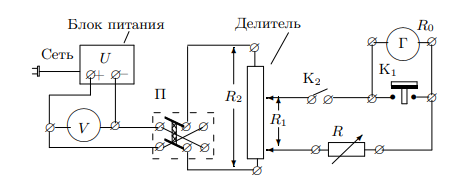
\includegraphics[width = 0.8 \textwidth]{УстновкаСтац.png}
    \caption{Схема установки для работы гальванометра в стационарном режиме}
\end{figure}
Схема для исследования гальванометра в стационарном режиме представлена на рис. 2. Постоянное напряжение $U \approx 1,5$ В снимается с блока питания и измеряетс я вольтметром $V$ . Ключ $\Pi$ позволяет менять направление тока через гальванометр $Г$, делитель напряжения -- менять величину тока в широких пределах. Ключ $\Pi$ служит для включения гальванометра, кнопка $К_1$ — для его успокоения. Магазин сопротивлений $R$ позволяет менять режим работы гальванометра от колебательного до апериодического. 

При малых $R_1$ сила тока, протекающего через гальванометр может быть вычислена по формуле:
\[I = U_0\frac{R_1}{R_2} \frac{1}{R + R_0}\]
где $U_0$ -- показания вольтметра, $R_1 / R_2$ -- положение делителя, \\ $R$ -- сопротивление магазина, $R_0$ -- внутреннее сопротивление гальванометра.

Угол отклонения рамки от положения равновесия измеряется с помощью осветителя, зеркальца, укреплённого на рамке, и шкалы, на которую отбрасывается луч света от зеркальца. Координата $x$ светового пятна на
шкале связана с углом отклонения рамки формулой
\[x = a \tan(2\varphi)\]
где $a$ -- расстояние от шкалы до зеркальца. При малых углах можно считать, что $\varphi = x/2a$. Динамическую постоянную выражаем как 
\[C_I = \frac{I}{x / 2a}\]

\textbf{Б. Определение критического сопротивления гальванометра, работающего в динамическом режиме}

Измерение критического сопротивления гальванометра можно выполнить с помощью той же цепи.

При больших $R$ свободное движение рамки имеет колебательный характер. С уменьшением $R$ затухание увеличивается, и колебательный режим переходит в апериодический.

Скорость затухания колебаний принято характеризовать логарифмическим \textit{декрементом затухания} $\Theta$:
\[\Theta = \ln{\frac{\varphi_n}{\varphi_{n + 1}}} = \gamma T\]
где $T$ -- период колебаний.

Измеряя зависимость логарифмического декремента затухания от сопротивления внешней цепи, можно найти $R_{кр}$, т. е. значение $R$, при
котором $\Theta \rightarrow \infty$. Подставляя значения получаем
\[\Theta = 2\pi \frac{\gamma}{\omega} = \frac{2\pi R_3}{\sqrt{(R_0 + R)^2 - R_3^2}}\]
где введено обозначение 
\[R_3 = \frac{(B S N)^2}{2\sqrt{JD}} = R_0 + R_{кр}\]
проведя простые преобразования получаем
\begin{equation}\label{eq: Theta^-2(R + R))}
    \frac{1}{\Theta^2} = \frac{(R + R_0)^2 }{4\pi^2 R_3^2} - \frac{1}{4\pi^2}
\end{equation}
для критического сопротивления получаем 
\[R_{кр} = \frac{1}{2 \pi} \sqrt{\frac{\Delta X}{\Delta Y}} - R_0\]

\textbf{В. Определение баллистической постоянной и критического сопротивления гальванометра, работающего в баллистическом режиме}

\begin{figure}[H]\label{fig: ustanovkaBallistRejim}
    \centering
    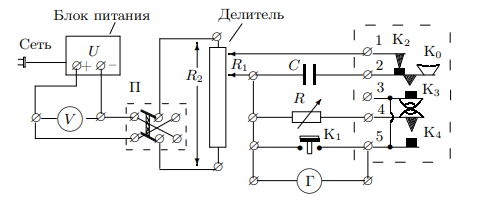
\includegraphics[width = 0.8 \textwidth]{УстновкаБаллист.png}
    \caption{Схема установки для определения баллистической постоянной}
\end{figure}

Для изучения работы гальванометра в режиме измерения заряда используется схема, представленная на рис. 3. Система ключей устроена так, что нормально ключ $K_2$ замкнут, $K_3$ и $K_4$ разомкнуты. При нажатии на кнопку $K_0$ сначала размыкается ключ $K_2$, затем замыкается $K_3$ и через некоторое время -- $K_4$. 

При нормальном положении кнопки $К_0$ конденсатор $C$ заряжается до напряжения
\[U_C = \frac{R_1}{R_2} \cdot U_0\]
Заряд конденсатора равен 
\[q = C U_C = \frac{R_1}{R_2} U_0 C\]

Первый отброс зайчика $l_{max}$ после нажатия на кнопку $К_0$ зависит от сопротивления внешней цепи, подключённой к гальванометру. Для определения
$R_{кр}$ используется то обстоятельство, что в критическом режиме максимальное отклонение зайчика в $e$ раз меньше, чем у гальванометра без затухания.

Следует понимать, что колебания рамки без затуханий наблюдать невозможно, так как всегда присутствует вязкое трение воздуха, а также трение в подвеске рамки. Величину максимального отклонения гальванометра без затухания $\varphi_0$ можно, однако, рассчитать, если при разомкнутой цепи измерены максимальное отклонение рамки $\varphi_1$ и логарифмический декремент затухания $\Theta_0$. При малом затухании ($\gamma \ll \omega_0$) получаем
\[\varphi_0 = \varphi_1 \cdot e^{\Theta_0 / 4}; \quad l_0 = l_1 \cdot e^{\Theta_0 / 4}\]
Баллистическая постоянная гальванометра определяется при критическом сопротивлении ($R = R_{кр}$)
\begin{equation}\label{eq: BallistConst}
    C_{Q_{кр}} = \frac{q}{\varphi_{max \text{ } кр}} = 2a\frac{R_1}{R_2} \frac{U_0 C}{l_{max \text{ } кр}}
\end{equation}

где $l_{max \text{ } кр}$ -- величина первого отброса в критическом режиме.

\textbf{Обработка данных}: 
\textbf{1) Определение динамической постоянной гальванометра:}. \\
Сначала исследуем зависимость угла отклонения рамки от значения постоянного тока в ней, с помощью этого рассчитаем динмаческую постоянную гальванометра. Некоторые параметры цепи: $R_1 / R_2 = 1 / 2000$, $U_0 = 66 / 150 \cdot 3 \text{ В} = (1,32 \pm 0,01)\text{ В}$, $R_0 = 500 \text{ Ом}$, $a = (103 \pm 1)\text{ см}$. По данным из таблицы ниже построим график зависимости $I$ от $x$. Подберём сопротивление так, чтобы луч света отклонялся на всю длину линейки. Это значение возьмём отправной точкой, дальше будем увеличивать значение сопротивления и замерять отклонение рамки. $R_{min} = 7800$ Ом.

\begin{table}[H]\label{tab: DataDynRejim}
    \centering
    \begin{tabular}{|c|c|c|c|}
        \hline
        {\color[HTML]{000000} $R$, Ом} & {\color[HTML]{000000} $x$, мм} & {\color[HTML]{000000} $R$, Ом} & {\color[HTML]{000000} $x$, мм} \\ \hline
        {\color[HTML]{000000} 7800}  & {\color[HTML]{000000} 250,0} & {\color[HTML]{000000} 33000} & {\color[HTML]{000000} 55,0} \\ \hline
        {\color[HTML]{000000} 12000} & {\color[HTML]{000000} 163,0} & {\color[HTML]{000000} 37200} & {\color[HTML]{000000} 49,5} \\ \hline
        {\color[HTML]{000000} 16200} & {\color[HTML]{000000} 120,0} & {\color[HTML]{000000} 41400} & {\color[HTML]{000000} 45,0} \\ \hline
        {\color[HTML]{000000} 20400} & {\color[HTML]{000000} 94,5}  & {\color[HTML]{000000} 45600} & {\color[HTML]{000000} 40,0} \\ \hline
        {\color[HTML]{000000} 24600} & {\color[HTML]{000000} 78,0}  & {\color[HTML]{000000} 49800} & {\color[HTML]{000000} 36,0} \\ \hline
        {\color[HTML]{000000} 28800} & {\color[HTML]{000000} 61,0}  & {\color[HTML]{000000} }      & {\color[HTML]{000000} }     \\ \hline
    \end{tabular}
    \caption{Данные при стационарном режиме работы гальванометра}
\end{table}

Коэффициент угла наклона прямой будем искать с помощью метода наименьших квадратов. 

\begin{figure}[H]\label{fig: I(x)_DynRejim}
    \centering
    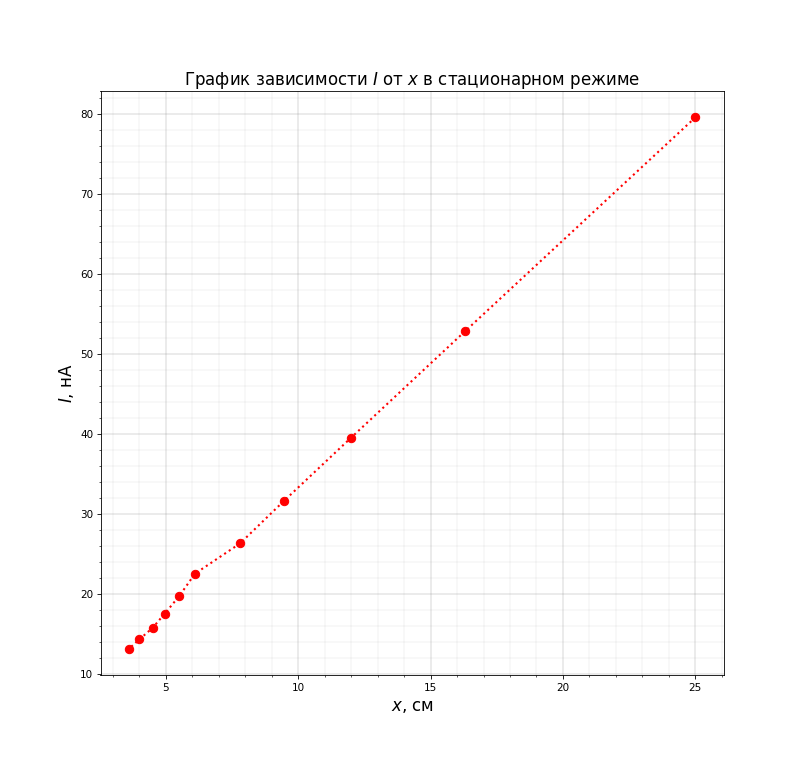
\includegraphics[width = \textwidth]{I(x)_DynRejim.png}
\end{figure}
\[k = (309,50 \pm 2,29) \text{ пА} / \text{ мм}  = \frac{C_I}{2 a}, \quad \varepsilon_k \approx 0,74 \%\]
\[C_I = (637,57 \pm 9,50) \text{ }\frac{пА}{мм / м}, \quad \varepsilon_{C_I}^2 = \varepsilon_k^2 + \varepsilon_a^2, \quad \varepsilon_{C_I} \approx 1,49 \%\]
%Здесь коэффициент наклона прямой был рассчитан следующим образом: так как $\varepsilon_{C_I} = \varepsilon_{C_I^-1}$, $\sigma_x = const$ (абсолютная погрешность измерения величины отклонения одинакова для всех точек), $\varepsilon_I = \varepsilon_{U_0} \approx 1,5 \%$, $\varepsilon_x \leq $

\textbf{2) Определение критического сопротивления гальванометра, работающего в динамическом режиме:} \\
Подберём значение сопротивления $R_{кр}$ -- наибольшее значение сопротивления, при котором при размыкании ключа $\Pi$ зайчик не переходит за нулевое значение. $R_{кр} = 8650$ Ом. Построим график зависимости $1  / \Theta^2 = f((R + R_0)^2)$ c  помощью которого и выражения \eqref{eq: Theta^-2(R + R))} найдём критическое сопротивление вторым способом, сравним результаты.

\begin{table}[H]\label{tab: DataTheta-1otR  R_02}
    \centering
    \begin{tabular}{|c|c|c|c|}
        \hline
        {\color[HTML]{000000} $R$, Ом} & {\color[HTML]{000000} $R_1 / R_2$} & {\color[HTML]{000000} $x_n$, мм} & {\color[HTML]{000000} $x_{n + 1}$, мм} \\ \hline
        {\color[HTML]{000000} 25950} & {\color[HTML]{000000} 1 / 1000} & {\color[HTML]{000000} 45}  & {\color[HTML]{000000} 4}  \\ \hline
        {\color[HTML]{000000} 30275} & {\color[HTML]{000000} 1 / 500}  & {\color[HTML]{000000} 84}  & {\color[HTML]{000000} 11} \\ \hline
        {\color[HTML]{000000} 34600} & {\color[HTML]{000000} 1 / 500}  & {\color[HTML]{000000} 82}  & {\color[HTML]{000000} 15} \\ \hline
        {\color[HTML]{000000} 38925} & {\color[HTML]{000000} 1 / 500}  & {\color[HTML]{000000} 79}  & {\color[HTML]{000000} 16} \\ \hline
        {\color[HTML]{000000} 43250} & {\color[HTML]{000000} 1 / 500}  & {\color[HTML]{000000} 73}  & {\color[HTML]{000000} 18} \\ \hline
        {\color[HTML]{000000} 47575} & {\color[HTML]{000000} 1 / 500}  & {\color[HTML]{000000} 73}  & {\color[HTML]{000000} 20} \\ \hline
        {\color[HTML]{000000} 51900} & {\color[HTML]{000000} 1 / 300}  & {\color[HTML]{000000} 115} & {\color[HTML]{000000} 35} \\ \hline
        {\color[HTML]{000000} 60550} & {\color[HTML]{000000} 1 / 300}  & {\color[HTML]{000000} 105} & {\color[HTML]{000000} 37} \\ \hline
        {\color[HTML]{000000} 69200} & {\color[HTML]{000000} 1 / 300}  & {\color[HTML]{000000} 96}  & {\color[HTML]{000000} 37} \\ \hline
        {\color[HTML]{000000} 77850} & {\color[HTML]{000000} 1 / 300}  & {\color[HTML]{000000} 89}  & {\color[HTML]{000000} 37} \\ \hline
        {\color[HTML]{000000} 86500} & {\color[HTML]{000000} 1 / 300}  & {\color[HTML]{000000} 82}  & {\color[HTML]{000000} 36} \\ \hline
    \end{tabular}
    \caption{Данные для нахождения критического сопротивления $R_{кр}$}
\end{table}
\begin{figure}[H]\label{fig: ThetaPow-2(R + R0)Pow2}
    \centering
    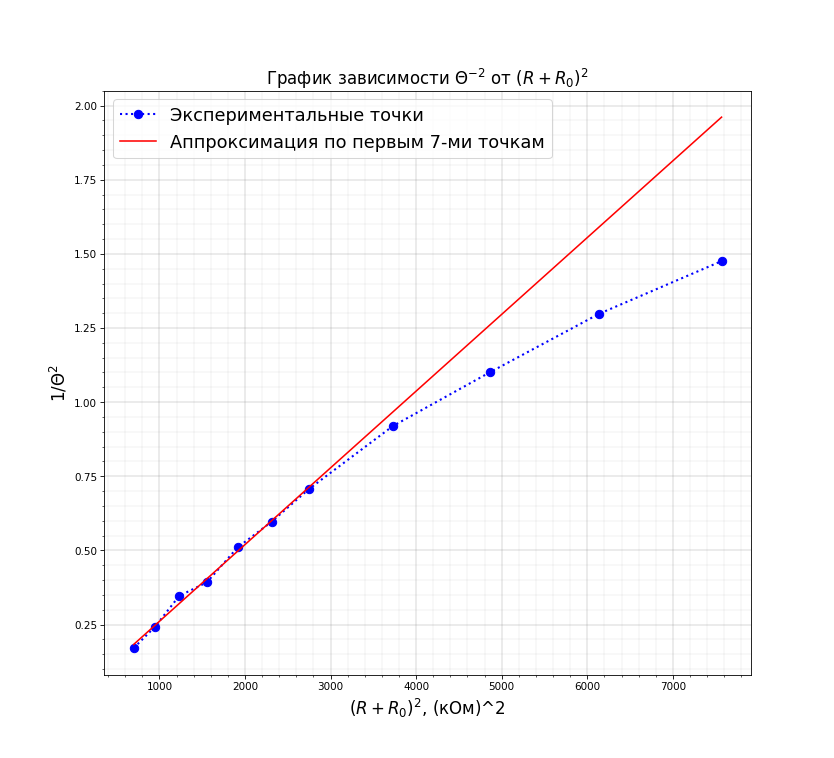
\includegraphics[width = \textwidth]{ThetaPow-2(R + R0)Pow2.png}
\end{figure}
\[k = (26,30 \pm 1,01) \cdot 10^{-11}, \quad \varepsilon_k \approx 3,84 \%\]
С помощью коэффициента наклона прямой найдём критической сопротивление $R_{кр}$ по формуле
\[R_{кр} = \frac{1}{2\pi} \sqrt{\frac{1}{k}} - R_0\]
\[R_{кр} = (9313,91 \pm 178,83) \text{ Ом}, \quad \varepsilon_{R_{кр}} = \frac{1}{2} \varepsilon_k \approx 1,92 \%\]
Подобранное значение $R_{кр1} = 8650,0$ Ом отличается от полученного вторым способом \\ $R_{кр2} = 9313,91$ Ом на $\approx 7 \%$.

Далее вычислим логарифмический декремент затухания $\Theta_0 = \ln ({x_n / x_{n + 1}})$ разомкнутого гальванометра, для этого измерим два последовательных максимума отклонения рамки
\[x_n = (209 \pm 1) \text{ }мм, \quad x_{n + 1} = (163 \pm 1) \text{ } мм\]
\[\sigma_{\Theta_0}^2 = (\frac{1}{{x_n}} - \frac{1}{x_{n + 1}})^2 \cdot \sigma_x^2\]
\[\Theta_0 = (248,6 \pm 1,4)\cdot 10^{-3}, \quad \varepsilon_{\Theta_0} \approx 0,56 \%\]

\textbf{3) Определение баллистической постоянной и критического сопротивления гальванометра, работающего в баллистическом режиме:} \\
Соберём цепь, представленную на рис. 3. Подберём положение делителя так, чтобы при замыкании ключа $К_0$ первый отброс $l_{1}$ соответствовал отклонению зайчика почти на всю шкалу. $R_1 / R_2 = 1 / 70$, $l_{1} = 250$ мм. Тогда величина первого отброса $l_0$ зайчика при незатухающих колебаниях выражается через $l_1$ как 
\[l_0 = l_1 \cdot e^{\Theta_0 / 4} = (265,99 \pm 1,06) \text{ мм}, \quad \varepsilon_{l_0} = \varepsilon_{l_{max \text{ } кр}} \approx 0,4 \%\]
\[l_{max \text{ кр}} = \frac{l_0}{e} = (97,85 \pm 0,39)\text{ мм}\]
\[\sigma_{l_0}^2 = \sigma_{l_1}^2 \cdot e^{\Theta_0 / 2} + \sigma_{\Theta_0}^2 \cdot \frac{l_1^2 e^{\Theta_0 / 2}}{16} \approx 1,13 \text{ } мм^2\]
Ёмкость конденсатора $C = 2$ мкФ. Затем будем менять сопротивление в цепи и записывать значение первого отброса зайчика. Данные представлены в таблице ниже.

\begin{table}[H]\label{tab: DataBallsitRejim}
    \centering
    \begin{tabular}{|c|c|c|c|}
        \hline
        {\color[HTML]{000000} $R$, Ом} & {\color[HTML]{000000} $l_{max}$, мм} & {\color[HTML]{000000} $R$, Ом} & {\color[HTML]{000000} $l_{max}$, мм} \\ \hline
        {\color[HTML]{000000} 50000} & {\color[HTML]{000000} 181} & {\color[HTML]{000000} 15000} & {\color[HTML]{000000} 130} \\ \hline
        {\color[HTML]{000000} 45000} & {\color[HTML]{000000} 179} & {\color[HTML]{000000} 10000} & {\color[HTML]{000000} 105} \\ \hline
        {\color[HTML]{000000} 40000} & {\color[HTML]{000000} 174} & {\color[HTML]{000000} 5000}  & {\color[HTML]{000000} 75}  \\ \hline
        {\color[HTML]{000000} 35000} & {\color[HTML]{000000} 168} & {\color[HTML]{000000} 4000}  & {\color[HTML]{000000} 65}  \\ \hline
        {\color[HTML]{000000} 30000} & {\color[HTML]{000000} 164} & {\color[HTML]{000000} 3000}  & {\color[HTML]{000000} 54}  \\ \hline
        {\color[HTML]{000000} 25000} & {\color[HTML]{000000} 151} & {\color[HTML]{000000} 2500}  & {\color[HTML]{000000} 48}  \\ \hline
        {\color[HTML]{000000} 20000} & {\color[HTML]{000000} 142} & {\color[HTML]{000000} 2000}  & {\color[HTML]{000000} 43}  \\ \hline
    \end{tabular}
    \caption{Зависимость максимального отклонения от сопротивления}
\end{table}
По результатам измерений построим график зависимости $l_{max}$ от $(R_0 + R)^{-1}$, с помошью этого графика найдём значение $R_{кр}$ третьим способом, сравним с двумя предыдущими.

\begin{figure}[H]\label{fig: L_max(R + R0)pow-1}
    \centering
    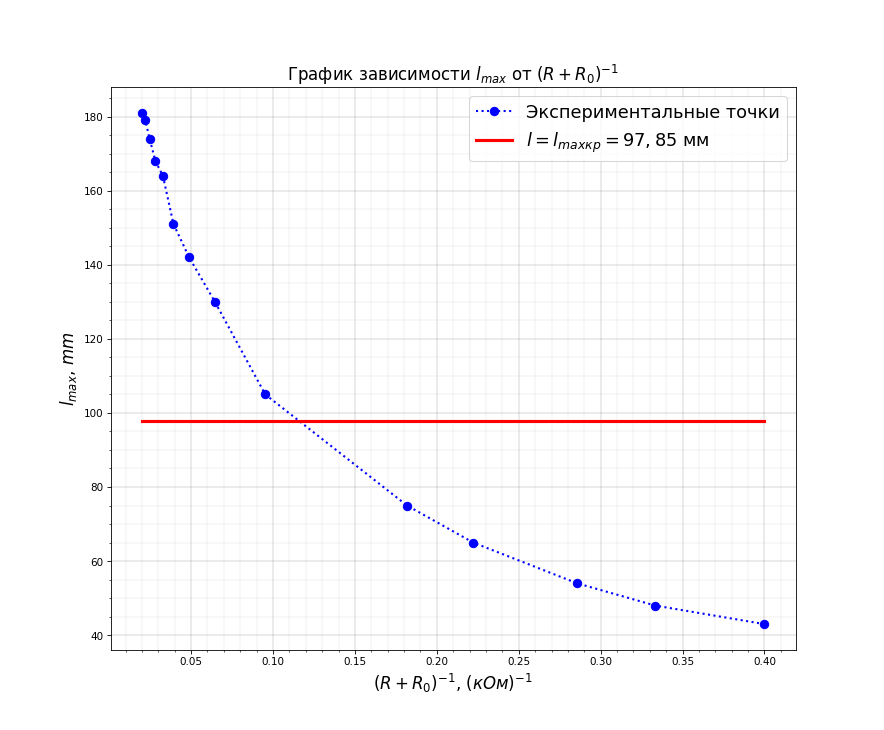
\includegraphics[width = \textwidth]{l_max(R + R0)pow-1_BallistRejim.png}
\end{figure}
Координата $x$ точки пересечения графика зависимости и прямой есть $1 / (R + R_0) = 0,000115 \text{ } (Ом)^{-1}$. Отсюда получаем, что 
\[R_{кр} = 8195,65 \text{ Ом}\]
Полученное значение $R_{кр}$ отличается от полученного подбором на $\approx 5\%$, от вычисленного вторым способом на $\approx 12\%$.

Зная значение для $l_0$, вычислим баллистическую постоянную по формуле \eqref{eq: BallistConst}
\[C_{Q_{кр}} = (7,94 \pm 0,10) \cdot 10^{-7} \text{ Кл} = (7,94 \pm 0,10) \cdot 10^{-10} \text{ } \frac{Кл}{мм / м}\]
\[\varepsilon_{C_{Q_{кр}}}^2 = \varepsilon_a^2 + \varepsilon_{l_{max \text{ кр}}}^2 + \varepsilon_{U}^2, \quad \varepsilon_{C_{Q_{кр}}} \approx 1,29 \%\]

Последним пунктом сравним период свободных колебаний гальванометра $T_0$ и его время релаксации $t = R_0 C$. Для этого сделаем несколько измерений периода колебаний рамки, затем найдем среднее значение и его ошибку.
\begin{table}[H]\label{tab: DataPeriodT}
    \centering
    \begin{tabular}{|c|c|c|c|}
        \hline
        {\color[HTML]{000000} №} & {\color[HTML]{000000} $T$, с} & {\color[HTML]{000000} №} & {\color[HTML]{000000} $T$, с} \\ \hline
        {\color[HTML]{000000} 1} & {\color[HTML]{000000} 5,54} & {\color[HTML]{000000} 5} & {\color[HTML]{000000} 5,77} \\ \hline
        {\color[HTML]{000000} 2} & {\color[HTML]{000000} 5,76} & {\color[HTML]{000000} 6} & {\color[HTML]{000000} 5,69} \\ \hline
        {\color[HTML]{000000} 3} & {\color[HTML]{000000} 5,63} & {\color[HTML]{000000} 7} & {\color[HTML]{000000} 5,33} \\ \hline
        {\color[HTML]{000000} 4} & {\color[HTML]{000000} 5,64} & {\color[HTML]{000000} }  & {\color[HTML]{000000} }     \\ \hline
    \end{tabular}
    \caption{Значения периода колебний рамки}
\end{table}
\[\sigma_{T_{ср}}^2 = \frac{\sum (T_i - T_{ср})^2}{N (N-1)}\]
\[T_{ср} = (5,623 \pm 0,057) \text{ c}, \quad \varepsilon_{T_{ср}} \approx 1,01\%\]
\[t = R_0 C = 1 \text{ мс} \ll T_{ср} = 5,623 \text{ c}\]

\textbf{Вывод}: В данной работе изучалась работа гальванометра. Были вычислены динамическая $C_I$ постоянная гальванометра и баллистическая $C_{Q_{кр}}$ в критическом режиме, а также, трёмя способами, было найдено внешнее сопротивление $R_{кр}$ цепи, при котором колебания проходили в критическом режиме ($\gamma \approx \omega_0$). Все значения отличаются друг от друга не более чем на $\approx 12\%$
\begin{table}[H]\label{tab: Vyvod}
    \centering
    \begin{tabular}{|c|ccc|c|c|}
        \hline
        {\color[HTML]{000000} } &
          \multicolumn{3}{c|}{{\color[HTML]{000000} $R_{кр}$, Ом}} &
          {\color[HTML]{000000} } &
          {\color[HTML]{000000} } \\ \cline{2-4}
        \multirow{}{}{{\color[HTML]{000000} $R_0$, Ом}} &
          \multicolumn{1}{c|}{{\color[HTML]{000000} Подбор}} &
          \multicolumn{1}{c|}{{\color[HTML]{000000} $1 / \Theta^2$}} &
          {\color[HTML]{000000} Балл} &
          \multirow{}{}{{\color[HTML]{000000} \begin{tabular}[c]{@{}c@{}}$C_I$, \\ $A / (мм / м)$\end{tabular}}} &
          \multirow{}{}{{\color[HTML]{000000} \begin{tabular}[c]{@{}c@{}}$C_{Q_{кр}}$, \\ $Кл / (мм / м)$\end{tabular}}} \\ \hline
        {\color[HTML]{000000} 500} &
          \multicolumn{1}{c|}{{\color[HTML]{000000} 8650}} &
          \multicolumn{1}{c|}{{\color[HTML]{000000} $9313,91 \pm 178,83$}} &
          {\color[HTML]{000000} 8195,65} &
          {\color[HTML]{000000} $(637,57\pm 9,50)\cdot 10^{-12}$} &
          {\color[HTML]{000000} $(7,94\pm 0,10) \cdot 10^{−10}$} \\ \hline
    \end{tabular}
    \caption{Результаты работы}
\end{table}

\end{document}
